%================================================================
% SLO
%----------------------------------------------------------------
% datoteka:   thesis_template
%
% opis:     predloga za pisanje diplomskega dela v formatu LaTeX na
%         Univerza v Ljubljani, Fakulteti za računalništvo in informatiko
%
% pripravili:   Matej Kristan, Zoran Bosnić, Andrej Čopar,
%          po začetni predlogi Gašperja Fijavža
%
% popravil:   Domen Rački, Jaka Cikač, Matej Kristan
%
% verzija:     30. september 2016 (dodan razširjeni povzetek)
%================================================================

%================================================================
% SLO: definiraj strukturo dokumenta
% ENG: define file structure
%================================================================
\documentclass[a4paper, 12pt]{book}

%================================================================
% SLO: Odkomentiraj "\SLOtrue " za izbiro slovenskega jezika
% ENG: Uncomment "\SLOfalse" to chose English languagge
%================================================================
\newif\ifSLO
\newif\ifTRACKEXIST
\newif\ifTRACKCS
\newif\ifPROGRAMMM
\newif\ifPROGRAMEMAI

% ---------------------------------------------------------------------------------------
% IMPORTANT: Adjust the thesis language, your study program and track within this block
% ---------------------------------------------------------------------------------------
% ** switch language ** %
% \SLOtrue % Enables Slovenian language
\SLOfalse  % Enables English language

% ** Switch programs: ** %

% ** Uncomment if Program: Computer Science, Track: Computer Science **%
\TRACKCStrue
\TRACKEXISTtrue

% ** Uncomment if Program: Computer Science, Track: Data Science **%
%\TRACKCSfalse
%\TRACKEXISTtrue

% ** Uncomment if Program: Multimedia **%
%\PROGRAMMMtrue
%\TRACKEXISTfalse

% ** Uncomment if Program: EMAI **%
%\PROGRAMEMAItrue
%\SLOfalse

% -------------------------------------------------------------------------------------------
% End of language, program and track adjustment
% -------------------------------------------------------------------------------------------

%================================================================
% SLO: vključi oblikovanje in pakete
% ENG: include design and packages
%================================================================
%----------------------------------------------------------------
% SLO: LaTeX paketi
% ENG: LateX packages
%----------------------------------------------------------------
% SLO: omogoča uporabo slovenskih (latinskih) črk kodiranih v formatu UTF-8
% ENG: enables the use of slovene (latin) caracters encoded in the UFT-8 format
\usepackage[utf8x]{inputenc}
%\inputencoding{utf8}
% SLO: naloži, med drugim, slovenske delilne vzorce
% ENG: loads, among others, slovene dividing patterns
\usepackage[slovene,english]{babel}
% SLO: poskrbi za postavitev strani
% ENG: takes care of the page layout
\usepackage{fancyhdr}
% SLO: za vlaganje slik različnih formatov
% ENG: for loading figures of different formats
\usepackage{graphicx}
\usepackage{tikz}
\usetikzlibrary{arrows.meta}
\usepackage{caption}
\captionsetup[figure]{labelfont=bf} % SLO: napis "Slika #" v krepkem tisku
% ENG: wirte "Figure #" caption in bold
\captionsetup[table]{labelfont=bf} % SLO: napis "Tabela #" v krepkem tisku
% ENG: wirte "Table #" caption in bold
% SLO: za pisanje psevdokode
% ENG: for writing pseudocode
\usepackage{algorithm}
\usepackage{algorithmic}
\floatname{algorithm}{\footnotesize Algorithm} % SLO: napis "Algoritem #" v krepkem tisku
% ENG: write "Algorithm #" caption in bold
% SLO: poveže reference slik/tabel in slike/tabele znotraj dokumenta
% ENG: links image/table references with the images/tables within the document
\usepackage[pdfa]{hyperref}
% SLO: pri kliku na referenco slike/tabele se postavi na vrh slike/tabele
% ENG: when clicking the image/table reference, position the focus on top of the image/table
\usepackage[all]{hypcap}
% SLO: omogoča, med drugim, definicjo in uporebo barve
% ENG: enables, among others, the definition and use of colors
\usepackage{xcolor}
%----------------------------------------------------------------
% SLO: dodatni paketi
% ENG: additional packages
%----------------------------------------------------------------
% SLO: omogoča večjo manipulacijo nad tabelami
% ENG: allows for greater manipulation of tables
\usepackage{booktabs}
% SLO: naloži dodatne simbole
% ENG: loads additional symbols
\usepackage{amssymb}
% SLO: omogoča, med drugim, sklicevanje na formule z eqref
% ENG: enables, among others, equation referencing with eqref
\usepackage{amsmath}
% Shared number formatting: decimal comma and thousands dot.
% Shared by the thesis and the Python-generated PGF figures.
% Enter numbers without grouping and with a decimal dot: \num{1234.56}.
\usepackage{siunitx}
\sisetup{
  output-decimal-marker = {,},
  group-separator = {.},
  group-minimum-digits = 4,
  group-digits = integer,
  range-phrase = {--},
  range-units = single
}

% SLO: omogoča komentiranje večjega dela teksta
% ENG: enables the commenting of larger text parts
\usepackage{verbatim}
\usepackage{listings}
% SLO: omogoča rotacijo PDF strani v ležeč položaj
% ENG: enables the rotation of a PDF page to landscape
\usepackage{pdflscape}
% SLO: omogoča barvanje vrstic in stolpcev tabel
% ENG: enables coloring of table rows and columns
\usepackage{colortbl}
\usepackage{url}

% TODO: Remove this in the final version
\usepackage{lipsum}

%================================================================
% SLO: nastavitve dokumenta
% ENG: document properties
%================================================================
% SLO: prilagoditev robov za tisk
% ENG: margin adjustments for printing
\addtolength{\marginparwidth}{-20pt}
\addtolength{\oddsidemargin}{40pt}
\addtolength{\evensidemargin}{-40pt}
% SLO: razmik med vrsticami
% ENG: line spacing
\renewcommand{\baselinestretch}{1.3}
% SLO: postavitev strani
% ENG: page layout
\renewcommand{\chaptermark}[1]{\markboth{\MakeUppercase{\thechapter.\ #1}}{}}
\renewcommand{\sectionmark}[1]{\markright{\MakeUppercase{\thesection.\ #1}}}
\renewcommand{\headrulewidth}{0.5pt} % Header rule
\renewcommand{\footrulewidth}{0pt} % Footer rule
%
\fancypagestyle{frontmatter}{%
  \fancyhf{} % Clear all headers and footers first
  \fancyhead[LE, RO]{\sl \thepage}
  %\fancyhead[LO]{\sl \rightmark}
  %\fancyhead[RE]{\sl \leftmark}
}
\fancypagestyle{mainmatter}{%
  \fancyhf{} % Clear all headers and footers first
  \fancyhead[LE,RO]{\sl \thepage}
  \fancyhead[LO]{\sl \rightmark}
  \fancyhead[RE]{\sl \leftmark}
}
% SLO: font za ime avtorja
% ENG: font for author name
\newcommand{\authorfont}{\Large}
% SLO: font za naslov diplomskega dela
% ENG: font for thesis title
\newcommand{\titlefont}{\LARGE\bf}
% SLO: globina kazala
% ENG: content depth
\setcounter{tocdepth}{1}
% SLO: definiraj ukaz za prazno stran
% ENG: define the command for empty page
\newcommand{\clearemptydoublepage}{\newpage{\pagestyle{empty}\cleardoublepage}}

% course title
\newcommand{\trackname}{!undefined!}

\newcommand{\BibTeX}{{\sc Bib}\TeX}


%----------------------------------------------------------------
% |||||||||||||||||||||| USTREZNO POPRAVI |||||||||||||||||||||||
% |||||||||||||||||||||| EDIT ACCORDINGLY |||||||||||||||||||||||
%----------------------------------------------------------------
\newcommand{\ttitle}{Analiza pristopov za pridobivanje informacij iz strukturiranih podatkov z uporabo
velikih jezikovnih modelov}
\newcommand{\ttitleEn}{Analysis of approaches for extracting information from structured data using large
language models}
\newcommand{\tsubject}{\ttitle}
\newcommand{\tsubjectEn}{\ttitleEn}
\newcommand{\tauthor}{Luka Pavićević}
\newcommand{\temail}{lp83866@student.uni-lj.si}
\newcommand{\myyear}{2026}
\newcommand{\tkeywords}{računalnik, računalnik, računalnik}
\newcommand{\tkeywordsEn}{computer, computer, computer}
\newcommand{\mysupervisor}{prof.~dr.\ Damjan Vavpotič}
% Uncomment and define the following definition if you have a co-supervisor
\newcommand{\mycosupervisor}{mag. Dragoslav Radin}

%%  Code publication under GNU
% NOTE: If you chose to publish the source code as part of the thesis, then put the url here and change the
% appropriate switch below !!
\newcommand{\linktosourcecode}{https://LINK-to-sourcecode-on-GIT}
\newif\ifCODEPUBLISHED

% Chosing the published code "true" will automatically generate the licence statement for the code on the licence page.
\CODEPUBLISHEDtrue % uncomment if the code is published
% \CODEPUBLISHEDfalse % uncomment if the code is not published
%% End of Code publication under GNU

% include formatted front pages

%----------------------------------------------------------------
% SLO: definiraj metapodatke za datoteko thesis_template.tex
% ENG: define metadata for the file thesis_template.tex
%----------------------------------------------------------------
%----------------------------------------------------------------
%  HYPERREF SETUP
% SLO: ustrezno popravi e-mail
% ENG: edit the e-mail accordingly
%----------------------------------------------------------------
\hypersetup{pdftitle={\ttitle}}
\hypersetup{pdfsubject=\ttitleEn}
\hypersetup{pdfauthor={\tauthor, \temail}}
\hypersetup{pdfkeywords=\tkeywordsEn}

%----------------------------------------------------------------
% define medatata
% SLO: ustrezno popravi e-mail
% ENG: edit the e-mail accordingly
%----------------------------------------------------------------
\def\Title{\ttitle}
\def\Author{\tauthor, \temail}
\def\Subject{\ttitleEn}
\def\Keywords{\tkeywordsEn}
\def\Org{Univerza v Ljubljani, Fakulteta za računalništvo in informatiko}

%%%%%%%%%%%%%%%%%%%%%%%%%%%%%%%%%%%%%%%%
% \convertDate converts D:20080419103507+02'00' to 2008-04-19T10:35:07+02:00
%%%%%%%%%%%%%%%%%%%%%%%%%%%%%%%%%%%%%%%%
\def\convertDate{%
  \getYear
}

{\catcode`\D=12
  \gdef\getYear D:#1#2#3#4{\edef\xYear{#1#2#3#4}\getMonth}
}
\def\getMonth#1#2{\edef\xMonth{#1#2}\getDay}
\def\getDay#1#2{\edef\xDay{#1#2}\getHour}
\def\getHour#1#2{\edef\xHour{#1#2}\getMin}
\def\getMin#1#2{\edef\xMin{#1#2}\getSec}
\def\getSec#1#2{\edef\xSec{#1#2}\getTZh}
\def\getTZh +#1#2{\edef\xTZh{#1#2}\getTZm}
\def\getTZm '#1#2'{%
  \edef\xTZm{#1#2}%
  \edef\convDate{\xYear-\xMonth-\xDay T\xHour:\xMin:\xSec+\xTZh:\xTZm}%
}

\expandafter\convertDate\pdfcreationdate

%%%%%%%%%%%%%%%%%%%%%%%%%%%%%%%%%%%%%%%%
% get pdftex version string
%%%%%%%%%%%%%%%%%%%%%%%%%%%%%%%%%%%%%%%%
\newcount\countA
\countA=\pdftexversion
\advance \countA by -100
\def\pdftexVersionStr{pdfTeX-1.\the\countA.\pdftexrevision}

%%%%%%%%%%%%%%%%%%%%%%%%%%%%%%%%%%%%%%%%
% XMP data
%%%%%%%%%%%%%%%%%%%%%%%%%%%%%%%%%%%%%%%%
\usepackage{xmpincl}
\includexmp{pdfa-1b}

%%%%%%%%%%%%%%%%%%%%%%%%%%%%%%%%%%%%%%%%
% pdfInfo
%%%%%%%%%%%%%%%%%%%%%%%%%%%%%%%%%%%%%%%%
\pdfinfo{%
  /Title    (\ttitle)h
  /Author   (\tauthor, \temail)
  /Subject  (\ttitleEn)
  /Keywords (\tkeywordsEn)
  /ModDate  (\pdfcreationdate)
  /Trapped  /False
}

%================================================================
% SLO: razno
% ENG: other
%================================================================
% SLO: nastavitev sklicevanj
% ENG: hyper referencing setup
\definecolor{black}{rgb}{0,0,0}
\hypersetup{
  colorlinks = true,
  linkcolor = black,
  citecolor = black,
  urlcolor = black
}

%----------------------------------------------------------------
% SLO: dodaj poti do datotek s slikami
% ENG: add paths to files containing figures
%----------------------------------------------------------------
\graphicspath{
  {figures/}
  {tables/}
}
%----------------------------------------------------------------
% SLO: moji paketi
% ENG: my packages
%----------------------------------------------------------------
% ...
%----------------------------------------------------------------
% SLO: moji konstrukti
% ENG: my constructs
%----------------------------------------------------------------
\newtheorem{izrek}{Izrek}[chapter]
\newtheorem{trditev}{Trditev}[izrek]
\newenvironment{dokaz}{\emph{Dokaz.}\ }{\hspace{\fill}{$\Box$}}

\newcommand{\CcImageCc}[1]{%
  
\includegraphics[scale=#1]{cc-licenca/cc_cc_30.pdf}%
}
\newcommand{\CcImageBy}[1]{%
  
\includegraphics[scale=#1]{cc-licenca/cc_by_30.pdf}%
}
\newcommand{\CcImageSa}[1]{%
  
\includegraphics[scale=#1]{cc-licenca/cc_sa_30.pdf}%
}

%================================================================
% SLO: začetne strani magistrskega dela
% ENG: fist pages of the master's thesis
%================================================================
\begin{document}
% SLO: prepreči težave s številkami strani v kazalu
% ENG: prevents problems with the page numbers in the contents page
\renewcommand{\thepage}{}

%----------------------------------------------------------------
% Language-dependent formatting
%----------------------------------------------------------------

\ifSLO
% SLO: definiraj slovensko besedo za kazalo
\renewcommand{\contentsname}{Kazalo}

% SLO: naslovnica
% select the course title if it exist

\ifPROGRAMEMAI
 
 \thispagestyle{empty}
	\begin{center}
		\noindent\makebox[\linewidth]{
\includegraphics[width=\linewidth]{style/Uni_logos.pdf}}

    	\vskip 7em
    	{\authorfont \tauthor}
		\vskip 2em
    	{\titlefont \ttitle \par}
        {\vskip 2em \textsc{MAGISTRSKO DELO\\[2mm]
		\textsc{SKUPNI ŠTUDIJSKI PROGRAM DRUGE STOPNJE UMETNA INTELIGENCA}
        }\par}
		{\vskip 5em \large Ljubljana, \myyear \par}
   \end{center}
 
   \vfill
   {\large {Univerza v Ljubljani}\par}
   {\large {Fakulteta za računalništvo in informatiko}\par}
   {\large {Mentor}: \mysupervisor \par}
   \ifdefined\mycosupervisor
	   {\large {Somentor}:  \mycosupervisor \par}
   \fi
\else
% ----------------
\ifTRACKEXIST
    \ifTRACKCS
        \renewcommand{\trackname}{Računalništvo in Informatika}
    \else
        \renewcommand{\trackname}{Podatkovne Vede}
    \fi
\fi

\ifPROGRAMMM
    \thispagestyle{empty}
    \begin{center}
        {\large\sc Univerza v Ljubljani\\Fakulteta za računalništvo in informatiko\\
            Fakulteta za elektrotehniko}
    	   \vskip 10em
    	   {\authorfont \tauthor \par}
    	   {\titlefont \ttitle \par}
        {\vskip 2em \textsc{MAGISTRSKO DELO\\[2mm]
        MAGISTRSKI ŠTUDIJSKI PROGRAM DRUGE STOPNJE\\MULTIMEDIJA
        }\par}
        \vfill\null
        {\large \textsc{Mentor}: \mysupervisor \par}
		\ifdefined\mycosupervisor
			{\large \textsc{Somentor}: \mycosupervisor \par}
		\fi
        {\vskip 2em \large Ljubljana, \myyear \par}
   \end{center}
\else
    \thispagestyle{empty}
	\begin{center}
            {\large\sc Univerza v Ljubljani\\Fakulteta za računalništvo in informatiko}
    	   \vskip 10em
    	   {\authorfont \tauthor \par}
    	   {\titlefont \ttitle \par}
        {\vskip 2em \textsc{MAGISTRSKO DELO\\[2mm]
        MAGISTRSKI ŠTUDIJSKI PROGRAM DRUGE STOPNJE\\RAČUNALNIŠTVO IN INFORMATIKA
        \ifTRACKEXIST
            \\Smer: \trackname
        \fi
        }\par}
        \vfill\null
        {\large \textsc{Mentor}: \mysupervisor \par}
		\ifdefined\mycosupervisor
			{\large \textsc{Somentor}: \mycosupervisor \par}
		\fi
        {\vskip 2em \large Ljubljana, \myyear \par}
   \end{center}
\fi 
% ---------------- 
\fi \clearemptydoublepage
% SLO: avtorske pravice
\thispagestyle{empty}
\vspace*{\fill}
{\noindent\footnotesize


\vspace*{5cm}
{\small \noindent
To delo je ponujeno pod licenco \textit{Creative Commons Priznanje avtorstva-Deljenje pod enakimi pogoji 4.0 Mednarodna (CC BY-SA 4.0)}.
To pomeni, da se lahko besedilo, slike, grafi in druge sestavine tega dela prosto delijo, reproducirajo, priobčujejo javnosti in predelujejo za vsak namen, tudi komercialno, če se jasno navede avtor (po možnosti tudi naslov in povezava do izvirnika), priloži povezava do licence, označijo morebitne spremembe, pri predelavah pa se uporabi enaka licenca (CC BY-SA 4.0). Licenca ne dovoljuje dodajanja dodatnih pravnih ali tehničnih omejitev in ne velja za dele, za katere nosilec pravic ni avtor.
Podrobnosti licence so dostopne na spletni strani \url{https://creativecommons.org}.

\begin{center}% 0.66 / 0.89 = 0.741573033707865
\CcImageCc{0.741573033707865}\hspace*{1ex}\CcImageBy{1}\hspace*{1ex}\CcImageSa{1}%
\end{center}
}


\ifCODEPUBLISHED
\vspace*{1.5cm}
{\small \noindent
Izvorna koda zaključnega dela, njeni rezultati in v ta namen razvita programska oprema je ponujena pod licenco GNU General Public License,
različica 3 (ali novejša). To pomeni, da se lahko prosto distribuira in/ali predeluje pod njenimi pogoji in je na voljo na \url{\linktosourcecode}.
Podrobnosti licence so dostopne na spletni strani \url{http://www.gnu.org/licenses/}.
}
\fi

}
\begin{center}
{\footnotesize{\sc \copyright \myyear\ \tauthor}}
\end{center}  \clearemptydoublepage
% SLO: izjava o avtorstvu (ni več del vezane izdaje, ločena oddaja)
% SLO: zahvala
\thispagestyle{empty}

\begin{center}
{\Large \textbf{\sc Zahvala}}
\end{center}
\vspace{0.5cm}

{\it\noindent
Na tem mestu zapišite, komu se zahvaljujete za izdelavo magistrske naloge. V zahvali se poleg mentorja spodobi omeniti vse, ki so s svojo pomočjo prispevali k nastanku vašega izdelka.

\vspace{0.5cm} \hfill \tauthor, \myyear
} \clearemptydoublepage
% SLO: posvetilo
\thispagestyle{empty}\mbox{}{\vskip0.20\textheight}\mbox{}\hfill\begin{minipage}{0.55\textwidth}%

Vsem rožicam tega sveta.\\\\
\textit{''The only reason for time is so that everything doesn't happen at once.''}
\flushright --- Albert Einstein
\normalfont\end{minipage} \clearemptydoublepage
\else

% ENG: title page ENG

\ifPROGRAMEMAI
 
 % in case of EMAI program, an additional front page will be generated
  
 \thispagestyle{empty}
	\begin{center}
		\noindent\makebox[\linewidth]{
\includegraphics[width=\linewidth]{style/EMAI_header.jpg}}

    	\vskip 4em
		{\titlefont \ttitleEn \par}
		
		\vskip 5em
    	{\authorfont \tauthor}
		
    	\vskip 7em
		  
 
   {\large {Supervisor}: \mysupervisor \par}
   \ifdefined\mycosupervisor
		{\large {Co-supervisor}:  \mycosupervisor \par}
   \fi
		
		{\vskip 5em \large Ljubljana, \myyear \par}
		
		 \vfill
       {\large {University of Ljubljana}\par}
   {\large {Faculty of Computer and Information Science}\par}
		
		
		
   \end{center}
 \newpage
 
 
 \thispagestyle{empty}
	\begin{center}
		\noindent\makebox[\linewidth]{
\includegraphics[width=\linewidth]{style/Uni_logos.pdf}}

    	\vskip 7em
    	{\authorfont \tauthor}
		\vskip 2em
    	{\titlefont \ttitleEn \par}
        {\vskip 2em \textsc{MASTER THESIS\\[2mm]
        ERASMUS MUNDUS JOINT MASTER IN ARTIFICIAL INTELLIGENCE
        }\par}
		{\vskip 5em \large Ljubljana, \myyear \par}
   \end{center}
 
   \vfill
   {\large {University of Ljubljana}\par}
   {\large {Faculty of Computer and Information Science}\par}
   {\large {Mentor}: \mysupervisor \par}
   \ifdefined\mycosupervisor
		{\large {Co-mentor}:  \mycosupervisor \par}
	\fi
	
\else
% ----------------
\ifTRACKEXIST
    \ifTRACKCS
        \renewcommand{\trackname}{Computer and Information Science}
    \else
        \renewcommand{\trackname}{Data Science}
    \fi
\fi
\ifPROGRAMMM
    \thispagestyle{empty}
	\begin{center}
        {\large\sc University of Ljubljana\\Faculty of Computer and Information Science\\
        Faculty of Electrical Engineering}
    	\vskip 10em
    	{\authorfont \tauthor \par}
    	{\titlefont \ttitleEn \par}
        {\vskip 2em \textsc{MASTER'S THESIS\\[2mm]
        THE 2nd CYCLE MASTER'S STUDY PROGRAMME\\MULTIMEDIA
        }\par}
        \vfill\null
        {\large \textsc{Supervisor}: \mysupervisor \par}
		\ifdefined\mycosupervisor
			{\large \textsc{Co-supervisor}:  \mycosupervisor \par}
		\fi
        {\vskip 2em \large Ljubljana, \myyear \par}
   \end{center}
\else
    \thispagestyle{empty}
	\begin{center}
        {\large\sc University of Ljubljana\\Faculty of Computer and Information Science}
    	\vskip 10em
    	{\authorfont \tauthor \par}
    	{\titlefont \ttitleEn \par}
        {\vskip 2em \textsc{MASTER'S THESIS\\[2mm]
        THE 2nd CYCLE MASTER'S STUDY PROGRAMME\\COMPUTER AND INFORMATION SCIENCE
        \ifTRACKEXIST
            \\Track: \trackname
        \fi
        }\par}
        \vfill\null
        {\large \textsc{Supervisor}: \mysupervisor \par}
		\ifdefined\mycosupervisor
			{\large \textsc{Co-supervisor}:  \mycosupervisor \par}
		\fi
        {\vskip 2em \large Ljubljana, \myyear \par}
    \end{center}
\fi
% ---------------- 
\fi \clearemptydoublepage
% ENG: title page SLO
% select the course title if it exist

\ifPROGRAMEMAI
 
 \thispagestyle{empty}
	\begin{center}
		\noindent\makebox[\linewidth]{
\includegraphics[width=\linewidth]{style/Uni_logos.pdf}}

    	\vskip 7em
    	{\authorfont \tauthor}
		\vskip 2em
    	{\titlefont \ttitle \par}
        {\vskip 2em \textsc{MAGISTRSKO DELO\\[2mm]
		\textsc{SKUPNI ŠTUDIJSKI PROGRAM DRUGE STOPNJE UMETNA INTELIGENCA}
        }\par}
		{\vskip 5em \large Ljubljana, \myyear \par}
   \end{center}
 
   \vfill
   {\large {Univerza v Ljubljani}\par}
   {\large {Fakulteta za računalništvo in informatiko}\par}
   {\large {Mentor}: \mysupervisor \par}
   \ifdefined\mycosupervisor
	   {\large {Somentor}:  \mycosupervisor \par}
   \fi
\else
% ----------------
\ifTRACKEXIST
    \ifTRACKCS
        \renewcommand{\trackname}{Računalništvo in Informatika}
    \else
        \renewcommand{\trackname}{Podatkovne Vede}
    \fi
\fi

\ifPROGRAMMM
    \thispagestyle{empty}
    \begin{center}
        {\large\sc Univerza v Ljubljani\\Fakulteta za računalništvo in informatiko\\
            Fakulteta za elektrotehniko}
    	   \vskip 10em
    	   {\authorfont \tauthor \par}
    	   {\titlefont \ttitle \par}
        {\vskip 2em \textsc{MAGISTRSKO DELO\\[2mm]
        MAGISTRSKI ŠTUDIJSKI PROGRAM DRUGE STOPNJE\\MULTIMEDIJA
        }\par}
        \vfill\null
        {\large \textsc{Mentor}: \mysupervisor \par}
		\ifdefined\mycosupervisor
			{\large \textsc{Somentor}: \mycosupervisor \par}
		\fi
        {\vskip 2em \large Ljubljana, \myyear \par}
   \end{center}
\else
    \thispagestyle{empty}
	\begin{center}
            {\large\sc Univerza v Ljubljani\\Fakulteta za računalništvo in informatiko}
    	   \vskip 10em
    	   {\authorfont \tauthor \par}
    	   {\titlefont \ttitle \par}
        {\vskip 2em \textsc{MAGISTRSKO DELO\\[2mm]
        MAGISTRSKI ŠTUDIJSKI PROGRAM DRUGE STOPNJE\\RAČUNALNIŠTVO IN INFORMATIKA
        \ifTRACKEXIST
            \\Smer: \trackname
        \fi
        }\par}
        \vfill\null
        {\large \textsc{Mentor}: \mysupervisor \par}
		\ifdefined\mycosupervisor
			{\large \textsc{Somentor}: \mycosupervisor \par}
		\fi
        {\vskip 2em \large Ljubljana, \myyear \par}
   \end{center}
\fi 
% ---------------- 
\fi \clearemptydoublepage
% ENG: copyright
\thispagestyle{empty}
\vspace*{\fill}
{\noindent\footnotesize


\vspace*{5cm}
{\small \noindent
This work is licensed under the \textit{Creative Commons Attribution–ShareAlike 4.0 International (CC BY-SA 4.0)} license.
This means that the text, images, graphs, and other components of this work may be freely shared, reproduced, made available to the public, and adapted for any purpose, including commercial use, provided that the author is clearly credited (preferably also the title and a link to the original), a link to the license is provided, any changes are indicated, and adaptations are distributed under the same license (CC BY-SA 4.0). The license does not permit the addition of extra legal or technological restrictions and does not apply to parts for which the rights holder is not the author.
Details of the license are available at \url{https://creativecommons.org}.

\begin{center}% 0.66 / 0.89 = 0.741573033707865
\CcImageCc{0.741573033707865}\hspace*{1ex}\CcImageBy{1}\hspace*{1ex}\CcImageSa{1}%
\end{center}
}

\ifCODEPUBLISHED
\vspace*{1.5cm}
{\small \noindent
The provided source code of the thesis, its results, and the software developed for this purpose are licensed under the GNU General Public License, version 3 (or later). This means they may be freely distributed and/or modified under its terms, and are available at \url{\linktosourcecode}. Details of the license are available on the website at \url{http://www.gnu.org/licenses/}.
}
\fi
   
}
\begin{center}
{\footnotesize{\sc \copyright \myyear\ \tauthor}}
\end{center}  \clearemptydoublepage
% ENG: declaration of authorship (not part of paper edition, turn in separately)
% ENG: acknowledgements
\thispagestyle{empty}

\begin{center}
{\Large \textbf{\sc Acknowledgments}}
\end{center}
\vspace{0.5cm}

{\it\noindent
Thanks to my mentor and co-mentor for providing me with thoughtful comments and guidance throughout this thesis.
Many thanks to my colleagues from DevRev for keeping me motivated. Finally, I thank my family for their continued support and encouragement throughout my studies.

\vspace{0.5cm} \hfill \tauthor, \myyear
} \clearemptydoublepage
% ENG: dedication
\thispagestyle{empty}\mbox{}{\vskip0.20\textheight}\mbox{}\hfill\begin{minipage}{0.55\textwidth}%

\textit{''Accept the things to which fate binds you, and love the people with whom fate brings you together,but do so with all your heart.''}
\flushright --- Marcus Aurelius
\normalfont\end{minipage} \clearemptydoublepage
\fi

%----------------------------------------------------------------
% SLO: kazalo
% ENG: contents
%----------------------------------------------------------------
\begingroup
\hypersetup{colorlinks=true,linkcolor=black}
\def\thepage{}
\tableofcontents{}
\clearemptydoublepage
\endgroup

\ifSLO
% SLO: seznam kratic
\chapter*{Seznam uporabljenih kratic}

\begin{tabular}{l|l|l}
  {\bf kratica} & {\bf angleško} & {\bf slovensko} \\ \hline
  % after \\: \hline or \cline{col1-col2} \cline{col3-col4} ...
  {\bf CA} & classification accuracy & klasifikacijska točnost \\
  {\bf DBMS} & database management system & sistem za upravljanje podatkovnih baz \\
  {\bf SVM} & support vector machine & metoda podpornih vektorjev \\
  ... & ... & ... \\
\end{tabular} \clearemptydoublepage
% SLO: glavne strani diplomskega dela
\else
% ENG: list of acronmys
\chapter*{List of used acronyms}

\begingroup
\renewcommand{\baselinestretch}{1}
\small
\noindent
\begin{tabular}{l|p{0.78\textwidth}}
  \textbf{Acronym} & \textbf{Meaning} \\ \hline
  \textbf{API} & Application Programming Interface \\
  \textbf{BLEU} & Bilingual Evaluation Understudy \\
  \textbf{BP} & Brevity Penalty \\
  \textbf{CI} & Confidence Interval \\
  \textbf{CLI} & Command-Line Interface \\
  \textbf{CPU} & Central Processing Unit \\
  \textbf{CSV} & Comma-Separated Values \\
  \textbf{CUDA} & Compute Unified Device Architecture \\
  \textbf{EM} & Exact Match \\
  \textbf{EX} & Execution Accuracy \\
  \textbf{GPT} & Generative Pre-trained Transformer \\
  \textbf{GPU} & Graphics Processing Unit \\
  \textbf{HTML} & HyperText Markup Language \\
  \textbf{IoT} & Internet of Things \\
  \textbf{JSON} & JavaScript Object Notation \\
  \textbf{KV} & Key--Value \\
  \textbf{LLM} & Large Language Model \\
  \textbf{LSTM} & Long Short-Term Memory \\
  \textbf{NDJSON} & Newline-Delimited JSON \\
  \textbf{NEM} & Normalized Exact Match \\
  \textbf{ONTO} & Object Notation for Token Optimization \\
  \textbf{ROUGE} & Recall-Oriented Understudy for Gisting Evaluation \\
  \textbf{SQL} & Structured Query Language \\
  \textbf{SVG} & Scalable Vector Graphics \\
  \textbf{TOML} & Tom's Obvious, Minimal Language \\
  \textbf{TOON} & Token-Oriented Object Notation \\
  \textbf{TTFT} & Time to First Token \\
  \textbf{VES} & Valid Efficiency Score \\
  \textbf{XML} & Extensible Markup Language \\
  \textbf{YAML} & YAML Ain't Markup Language \\
\end{tabular}
\par
\endgroup
 \clearemptydoublepage
\fi

\frontmatter
\pagestyle{frontmatter}
\setcounter{page}{1} %
\renewcommand{\thepage}{}       % preprecimo težave s številkami strani v kazalu

% Include extended abstract [Razširjeni povzetek v slovenščini-- le za dela pisana v angleščini]
\ifSLO
% include Slovenian abstract
%---------------------------------------------------------------
% SLO: slovenski povzetek
% ENG: slovenian abstract
%---------------------------------------------------------------
\selectlanguage{slovene} % Preklopi na slovenski jezik
\addcontentsline{toc}{chapter}{Povzetek}
\chapter*{Povzetek}

\noindent\textbf{Naslov:} \ttitle
\bigskip

Magistrsko delo primerja neposredno sklepanje iz konteksta in pretvorbo besedila v SQL pri pridobivanju
informacij iz strukturiranih podatkov z velikimi jezikovnimi modeli. Ovrednotili smo \num{10} lokalno
nameščenih modelov z odprtimi utežmi in \num{6} serializacijskih formatov na podatkovnih bazah iz zbirke
Spider in podvzorčenih bazah iz zbirke BIRD. Če neuspele zagone in zagone s preseženim kontekstnim oknom
ovrednotimo z ničlo, je pretvorba besedila v SQL najboljši neposredni format v povprečnem normaliziranem
natančnem ujemanju v celoti na kohorti odgovorljivih vprašanj presegla za \num{46.5} oziroma \num{44.7}
odstotne točke, na preseku s kontekstno ustrezno kohorto, kjer vse konfiguracije ustrezajo kontekstnemu
oknu, pa za \num{45.8} oziroma \num{38.0} odstotne točke; pri tem je bila ustrezna prednost po meri
BERTScore na tem preseku le \num{4.9} oziroma \num{2.0} odstotne točke. Primerjave operativne učinkovitosti
na kontekstno ustrezni kohorti so pri pretvorbi besedila v SQL pokazale manjšo porabo vhodnih žetonov in
krajši povprečni odzivni čas. Med neposrednimi formati je bil najučinkovitejši CSV, sledil mu je TOON
(Token-Oriented Object Notation). Ugotovitve so podlaga za odločitveni okvir, ki daje prednost izbiri
metode pred serializacijo ter priporoča pretvorbo besedila v SQL, kadar je izvajanje poizvedb SQL na voljo
in primerno za nalogo.

\subsection*{Ključne besede}
\textit{\tkeywords}
\clearemptydoublepage

% include English abstract
 %---------------------------------------------------------------
% SLO: angleški povzetek
% ENG: english abstract
%---------------------------------------------------------------
\selectlanguage{english} % Preklopi na angleški jezik
\addcontentsline{toc}{chapter}{Abstract}
\chapter*{Abstract}

\noindent\textbf{Title:} \ttitleEn
\bigskip

Extracting information from structured data using large language models requires balancing answer quality,
response latency, and resource consumption. This thesis investigates how the extraction method and data
serialization format influence these requirements. We compared direct context inference, in which models
answer questions from serialized database contents, with text-to-SQL, in which models generate queries
executed by a database engine. The evaluation used \num{10} locally deployed open-weight models,
\num{6} serialization formats, and databases from Spider and a subsampled version of BIRD. We measured
reference-answer agreement, token consumption, and response latency. Text-to-SQL achieved higher mean
agreement than every direct-inference format, exceeding the strongest direct format in normalized exact
match by \num{46.5} percentage points on Spider and \num{44.7} percentage points on sampled BIRD.
In separate comparisons on shared context-fit workloads, it also required fewer input tokens and had
lower mean response latency. For direct inference on flat relational tables, CSV required the fewest
input tokens and had the lowest mean latency, with Token-Oriented Object Notation (TOON) a close
alternative; more verbose formats offered no consistent advantage in answer agreement. These findings
inform a decision framework that prioritizes extraction-method selection before serialization
optimization and supports text-to-SQL as the preferred method when SQL execution is available and
the task can be expressed as a query.

\subsection*{Keywords}
\textit{\tkeywordsEn}
\clearemptydoublepage

\else
% include English abstract
 %---------------------------------------------------------------
% SLO: angleški povzetek
% ENG: english abstract
%---------------------------------------------------------------
\selectlanguage{english} % Preklopi na angleški jezik
\addcontentsline{toc}{chapter}{Abstract}
\chapter*{Abstract}

\noindent\textbf{Title:} \ttitleEn
\bigskip

Extracting information from structured data using large language models requires balancing answer quality,
response latency, and resource consumption. This thesis investigates how the extraction method and data
serialization format influence these requirements. We compared direct context inference, in which models
answer questions from serialized database contents, with text-to-SQL, in which models generate queries
executed by a database engine. The evaluation used \num{10} locally deployed open-weight models,
\num{6} serialization formats, and databases from Spider and a subsampled version of BIRD. We measured
reference-answer agreement, token consumption, and response latency. Text-to-SQL achieved higher mean
agreement than every direct-inference format, exceeding the strongest direct format in normalized exact
match by \num{46.5} percentage points on Spider and \num{44.7} percentage points on sampled BIRD.
In separate comparisons on shared context-fit workloads, it also required fewer input tokens and had
lower mean response latency. For direct inference on flat relational tables, CSV required the fewest
input tokens and had the lowest mean latency, with Token-Oriented Object Notation (TOON) a close
alternative; more verbose formats offered no consistent advantage in answer agreement. These findings
inform a decision framework that prioritizes extraction-method selection before serialization
optimization and supports text-to-SQL as the preferred method when SQL execution is available and
the task can be expressed as a query.

\subsection*{Keywords}
\textit{\tkeywordsEn}
\clearemptydoublepage

% include Slovenian abstract
%---------------------------------------------------------------
% SLO: slovenski povzetek
% ENG: slovenian abstract
%---------------------------------------------------------------
\selectlanguage{slovene} % Preklopi na slovenski jezik
\addcontentsline{toc}{chapter}{Povzetek}
\chapter*{Povzetek}

\noindent\textbf{Naslov:} \ttitle
\bigskip

Magistrsko delo primerja neposredno sklepanje iz konteksta in pretvorbo besedila v SQL pri pridobivanju
informacij iz strukturiranih podatkov z velikimi jezikovnimi modeli. Ovrednotili smo \num{10} lokalno
nameščenih modelov z odprtimi utežmi in \num{6} serializacijskih formatov na podatkovnih bazah iz zbirke
Spider in podvzorčenih bazah iz zbirke BIRD. Če neuspele zagone in zagone s preseženim kontekstnim oknom
ovrednotimo z ničlo, je pretvorba besedila v SQL najboljši neposredni format v povprečnem normaliziranem
natančnem ujemanju v celoti na kohorti odgovorljivih vprašanj presegla za \num{46.5} oziroma \num{44.7}
odstotne točke, na preseku s kontekstno ustrezno kohorto, kjer vse konfiguracije ustrezajo kontekstnemu
oknu, pa za \num{45.8} oziroma \num{38.0} odstotne točke; pri tem je bila ustrezna prednost po meri
BERTScore na tem preseku le \num{4.9} oziroma \num{2.0} odstotne točke. Primerjave operativne učinkovitosti
na kontekstno ustrezni kohorti so pri pretvorbi besedila v SQL pokazale manjšo porabo vhodnih žetonov in
krajši povprečni odzivni čas. Med neposrednimi formati je bil najučinkovitejši CSV, sledil mu je TOON
(Token-Oriented Object Notation). Ugotovitve so podlaga za odločitveni okvir, ki daje prednost izbiri
metode pred serializacijo ter priporoča pretvorbo besedila v SQL, kadar je izvajanje poizvedb SQL na voljo
in primerno za nalogo.

\subsection*{Ključne besede}
\textit{\tkeywords}
\clearemptydoublepage


% %  \cleardoublepage
% \let\oldthesection=\thesection %Special section numbering for this chapter - remember default one
% \let\oldthesubsection=\thesubsection
% \renewcommand{\thesection}{\Roman{section}} %Special section numbering for this chapter
% \renewcommand{\thesubsection}{\thesection.\Roman{subsection}}

% % set roman page numbering
% \pagenumbering{roman}
% % set slovene language
% \selectlanguage{slovene}
% % insert extended abstract
% \chapter{Razširjeni povzetek}

\section{Kratek pregled sorodnih del}

\section{Predlagana metoda}

\section{Eksperimentalna evaluacija}

\section{Sklep}


% \let\thesection=\oldthesection % Restore default section numbering
% \let\thesubsection=\oldthesubsection
\fi

%----------------------------------------------------------------
% SLO: Preklopi izbrani jezik
% ENG: Switch to chosen language
%----------------------------------------------------------------
\ifSLO
\selectlanguage{slovene} % Preklopi na slovenski jezik
\else
\selectlanguage{english}  % Switch to english language
\fi

% SLO: vklopi številčenje poglavji, ponastavi številčenje strani in uporabi arabske številkami za številčenje strani
% ENG: turns on chapter numbering, resets page numbering and uses arabic numerals for page numbers
\mainmatter
\pagestyle{mainmatter}
\setcounter{page}{1}
\pagestyle{fancy}


%================================================================
% ENG: main pages of the thesis
%================================================================

%----------------------------------------------------------------
% Poglavje (Chapter) 1
%----------------------------------------------------------------
\chapter{Uvod}
\label{ch:uvod}

Datoteka {\tt magistrska\_naloga.tex} na kratko opisuje, kako se pisanja magistrskega dela lotimo z uporabo
programskega pateka \LaTeX. V tem dokumentu bomo predstavili nekaj njegovih prednosti in hib. Kar se slednjih
tiče, mi pride na misel ena sama. Ko se srečamo z njim, nam izgleda kot kislo jabolko, nismo prepričani, da
bi želeli vanj ugrizniti. Lahko pa z njim pripravimo odličen zavitek ali pa pridemo na okus.

V Poglavju~\ref{ch:uvod} bomo na hitro spoznali besedilne konstrukte kot so izreki, enačbe in dokazi. Naučili
se bomo, kako se na njih sklicujemo. V Poglavju~\ref{ch:sklicevanje} se bomo srečali s sklicevanjem na
besedilne konstrukte. Poglavje~\ref{ch:plovke} bo predstavilo vključevanje plovk: slik in tabel. V
Poglavju~\ref{ch3} se bomo srečali s sklicevanjem na literaturo.
Sledil bo samo še zaključek.

Bodite pozorni, da se v glavni mapi nahajata še datoteki \verb+ declaration.tex+ in \verb+ izjava.tex+. Ti
datoteki se ločeno prevedeta, ju podpišete in oddate v referat ločeno od magistrske naloge.
%----------------------------------------------------------------
% Poglavje (Chapter) 2
%----------------------------------------------------------------
\chapter{Related work}
\label{ch:related_work}

The research into the relationship between data serialization and performance of LLMs has grown from a prompt
engineering concern, to the important questions a lot of experts are asking. As LLMs are increasingly
integrated into enterprise pipelines, the way data is structured, be it JSON, XML, CSV, Markdown, has been
shown to hold a significant influence over the overall performance of the models (cost, accuracy, efficiency).
This is not a mere question of our format preference, the benchmarks such as StrucText-Eval
\cite{struct-text-eval} has given us insight how such formats influence the overall accuracy of the models.

\section{A Survey of Structured Data Representations}

To understand how format influences models, it's paramount to have a way of organizing structured data
representations that we are going to be using. We can identify several main categories of data representation, as
shown by the StrucText-Eval \cite{struct-text-eval}. These categories show the range of data formats, from
those that are strictly structured to those that are semi-structured. Structured data is consistent and
organized. This makes it easy for computers
to process, but it also creates some overhead when LLMs are tokenizing the data. The most common
classification system divides these into four main types:
% TODO: Add citations for all of the data formats !!!
\begin{itemize}
  \item \textbf{Tree and Tabular Formats:} These includes CVS files and custom hierarchical notation. In these
    formats, relationships are defined either by positional alignment (as in CSV) or explicit pointers (as in
    tree structures). However, CSV fundamentally cannot represent nested structures, limiting its
    applicability to flat tabular data.
  \item \textbf{Object Notation:} This category represents the most common data interchange languages in
    software development, notably JSON (JavaScript Object Notation), YAML (YAML Ain't Markup Language), and
    TOML. These formats rely on key-value pairs and nesting to represent multi-dimensional data
  \item \textbf{Markup Languages:} Semi-structured data types like Markdown, LaTeX, and Org represent
    information in a human-readable form while embedding structural metadata (headings, lists, and semantic
    tags). Markdown has become the de facto standard for general-purpose LLM interactions due to its presence
    in training data.
  \item \textbf{Code Based Formats:} These include HTML, JSX, SVG, and XML. These formats are special
    because they are measured not only by how well they follow the rules of language, but also by how well they
    can create a visual or logical output that meets the requirements of the user.

\end{itemize}

% The categorization of these formats is critical because each imposes a different "tokenization
% overhead." For instance, JSON requires significant structural punctuation (braces, quotes, colons), whereas
% YAML relies on whitespace and indentation. The structural density of a format influences the model's ability
% to maintain context over long sequences, as redundant tokens can "dilute" the attention allocated to the
% actual semantic content.

\section{Token Efficiency and Economic Impact of Data Serialization}

The choice of data format has direct impact on the computational cost of LLMs. Format verbosity determines
token token usage of the model, and this has a knock on effect for other factors, such as latency, API cost,
and effective context window.

Formats like JSON and XML are inefficient with token usage, as they have been designed for data exchange
between information systems, where self description and compatibility were more important than their
verbosity. These formats are designed in such a way that each fields carries its own description, through
repeated key words, which create overhead when working with LLMs. The experiments performed in \cite{}, were
carried out across $1.000$ IoT telemetry records. They have shown that majority of encoding tokens used for
encoding data in the JSON format is used up by field names and punctuation ($60.500$ tokens), while the
actual semantic values take up only $14.274$ tokens, out of $79.774$ tokens. This overhead is problematic in
the current age, as most pricing is done based on the input and output tokens used, with this higher token
usage directly translates to higher operational costs for the users. Also in the same experiment it was shown
that reduction in tokens used directly correlates to lower latency, when compared to their custom ONTO format.

In order to address these inefficiencies, there have been multiple efforts aimed at them, in form of ONTO
(Object Notation for Token Optimization) and TOON (Token Optimized Object Notation). Both formats are
oriented at fixing the problem of repeated schema for each record, they fix this by declaring all the fields
only once at the top of the record, and values are arrange in pipe delimited rows with indentation based
hierarchy. Both of these models claim to use significantly less tokens (TOON $39.9\%$ fewer tokens compared
to JSON, and ONTO $46-51\%$ compared to JSON ) while minimal impacts on accuracy.

%----------------------------------------------------------------
% Poglavje (Chapter) 3
%----------------------------------------------------------------
\chapter{Plovke: slike in tabele}
\label{ch:plovke}

Slike in daljše tabele praviloma vključujemo v dokument kot plovke. Pozicija plovke v končnem izdelku ni
pogojena s tekom besedila, temveč z izgledom strani. \LaTeX\ bo skušal plovko postaviti samostojno, praviloma
na vrh strani, na kateri se na takšno plovko prvič sklicujemo. Pri tem pa bo na vsako stran končnega izdelka
želel postaviti tudi sorazmerno velik del besedila. V skrajnem primeru, če imamo res preveč plovk, se bo
odločil za stran popolnoma zapolnjeno s plovkami.

\section{Formati slik}
Bitne slike, vektorske slike, kakršnekoli slike, z \LaTeX{}om lahko vključimo vse.
Slika~\ref{pic1} je v {\tt .pdf} formatu.
\begin{figure}
  \begin{center}
    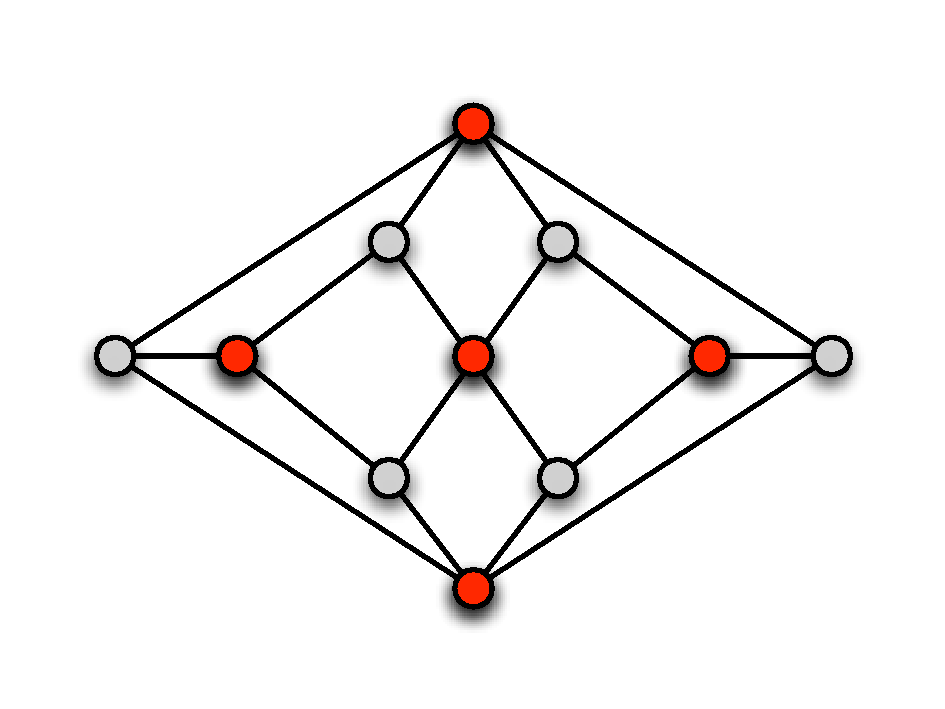
\includegraphics[width=10cm]{pic1.pdf}
  \end{center}
  \caption{Herschelov graf, vektorska grafika.}
  \label{pic1}
\end{figure}
Pa res lahko vključimo slike katerihkoli formatov? Žal ne. Programski paket \LaTeX\ lahko uporabljamo v več
dialektih. Ukaz {\tt latex} ne mara vključenih slik v formatu Portable Document Format {\tt .pdf}, ukaz {\tt
pdflatex} pa ne prebavi slik v Encapsulated Postscript Formatu {\tt .eps}.
Strnjeno v Tabeli~\ref{tbl:1}.

\begin{table}
  \caption{}
  \begin{center}
    \begin{tabular}{l|ccc}
      ukaz/format & {\tt .pdf} & {\tt .eps} & ostali formati \\ \hline
      {\tt pdflatex} & da & ne & da \\
      {\tt latex}   & ne & da  & da
    \end{tabular}
  \end{center}
  \label{tbl:1}
\end{table}

Nasvet? Odločite se za uporabo ukaza {\tt pdflatex}. Vaš izdelek bo brez vmesnih stopenj na voljo v {.pdf}
formatu in ga lahko odnesete v vsako tiskarno. Če morate na vsak način vključiti sliko, ki jo imate v {\tt
.eps} formatu, jo vnaprej pretvorite v alternativni format, denimo {\tt .pdf}.

Včasih se da v okolju za uporabo programskega paketa \LaTeX\ nastaviti na kakšen način bomo prebavljali
vhodne dokumente. Spustni meni na Sliki~\ref{pic2} odkriva uporabo \LaTeX{}a v njegovi pdf inkarnaciji ---
{\tt pdflatex}.
\begin{figure}
  \begin{center}
    
\includegraphics[width=10cm]{pic2.png}
  \end{center}
  \caption{Kateri dialekt uporabljati?}
  \label{pic2}
\end{figure}
Vključena Slika~\ref{pic2} je seveda bitna.

%----------------------------------------------------------------
% Poglavje (Chapter) 4
%----------------------------------------------------------------
\chapter{Implementation}
\label{ch:implementation}

\lipsum

%----------------------------------------------------------------
% Poglavje (Chapter) 5
%----------------------------------------------------------------
\chapter{Kaj pa literatura?}
\label{ch3}
Kot smo omenili že v uvodu, je pravi način za citiranje literature uporaba \BibTeX{}a~\cite{ubi}.
Programski paket \LaTeX je prvotno predstavljen v priročniku~\cite{Lamport} in je v resnici nadgradnja
sistema \TeX\ avtorja Donalda Knutha, znanega po denimo, če izpustim njegovo umetnost programiranja,
Knuth-Bendixovem algoritmu~\cite{Knuth}.

Vsem raziskovalcem s področja računalništva pa svetujem v branje mnenje L.\ Fortnowa~\cite{Fortnow}.
\chapter{Discussion}
\label{ch:discussion}

This chapter interprets the findings in Chapter~\ref{ch:results} and develops a framework for selecting an
extraction method and, where needed, a serialization format. The populations follow
Section~\ref{sec:analysis-cohorts}: retrieval accuracy uses the answerable cohort, while comparative
operational efficiency uses the context-fit cohort. These overlapping but different populations support
separate interpretations, not a jointly measured quality--resource frontier.

\section{Interpretation of the main findings}
\label{sec:main-findings-interpretation}

\subsection{Pipeline selection and database size}
\label{sec:pipeline-size-interpretation}

The paired comparisons in Section~\ref{sec:common-cohort-comparison} favour Text-to-SQL for reference-answer
agreement across metrics on the evaluated relational workloads. For example, on Spider, even JSON, the direct
format with the highest mean NEM, had a paired JSON-minus-SQL difference of \num{-0.465}
(\numrange{-0.507}{-0.422}). The corresponding comparisons on sampled BIRD also favoured SQL.
Delegating retrieval and aggregation to the database engine was therefore more effective than asking the
model to derive the answer directly from the serialized records under these conditions. This supports
considering the extraction method before optimizing its input representation.

The size-tier results strengthen this interpretation. In
Section~\ref{sec:pipeline-accuracy-by-database-size}, every paired direct-minus-SQL interval was below zero
for all three metrics in every tier, including small databases. Small size establishes potential
direct-context feasibility, but does not by itself justify preferring Direct Context Inference. Both
pipelines had lower mean NEM in the large tier, and the size of the gap changed differently across metrics.
The evidence does not support a simple rule that one method becomes preferable at a particular tier
boundary.

The negative database-size associations in Section~\ref{sec:direct-results} include zero scores for context
failures, rather than isolating accuracy among feasible requests. Size also varied with domain, schema, and
questions. In the pooled tiers, all small and medium databases
were from Spider, while all sampled BIRD databases belonged to the large tier. Dataset composition is
therefore an additional confounder when comparing tiers. Neither these comparisons nor the separate
within-dataset associations establish a causal effect of size. They instead show why context capacity and
answer quality must be considered separately. For relational tasks that can be expressed in SQL and whose
infrastructure permits its use, the results support Text-to-SQL as the first candidate; the deployment
conditions are specified in Section~\ref{sec:decision-framework}.

\subsection{Serialization trade-offs}

CSV is a practical starting representation for flat Direct Context Inference inputs. It required the
fewest payload tokens on average in Section~\ref{sec:serialization-results}, while TOON remained close.
The request-level comparison in Section~\ref{sec:direct-results} also showed lower input-token use and
shorter mean latency for these compact formats than for the more verbose alternatives. Much of the timing
difference occurred in TTFT, so the benefit primarily concerned processing the supplied input rather than
shortening the generated answer. Compactness also extended the set of databases that could potentially
be supplied to the model.

However, token efficiency does not establish a universal agreement ranking. JSON had the highest observed
direct NEM mean on Spider, but its paired advantage over CSV was only \num{0.57} percentage points
(\numrange{-1.21}{2.34}). This does not establish a clear advantage, nor does it prove equivalence. CSV
had the highest direct mean BERTScore and ROUGE-L on Spider and the highest means on all three measures
on sampled BIRD, with TOON generally competitive. Format selection should therefore consider the paired
evidence and its uncertainty, not only the ordering of means.

These findings favour avoiding unnecessary verbosity, rather than conversion at any price. Representational
fidelity remains a prerequisite: reducing tokens is not useful if it removes relationships needed for the
answer. The experiment evaluated serialized relational tables, not nested-data retrieval. Moreover,
payload counts describe the data alone, not a complete request, and arithmetic means can be dominated by
one large database. Actual context feasibility must be checked for the selected representation and model.
The framework gives the conditional rules for preserving structure or retaining an existing format.

\subsection{Model and dataset effects}

Model selection mattered within both pipelines, but nominal parameter count was not an isolated explanatory
variable. The family-specific comparisons in Figures~\ref{fig:direct-accuracy-by-model-size} and
\ref{fig:text-to-sql-accuracy-by-model-size} showed different gains across variants and datasets. In
Text-to-SQL, the Qwen comparisons showed substantial improvements from the smallest variants, with much
of the observed gain occurring by 4B. This does not imply that the same scaling pattern holds for every
family or application. In Direct Context Inference, the larger Gemma and Ministral variants did not show
clear NEM improvements in the reported sampled-BIRD comparisons.

Architecture and training also changed between variants. Gemma~4 26B-A4B, for example, is positioned at
its total nominal parameter count in the figures, not its approximately 4B active parameters. Model choices
therefore require measured performance rather than a parameter-count threshold.

Lower agreement on sampled BIRD in both pipelines further shows that the workload matters. Its data,
schemas, questions, and sampling procedure differ from Spider, so the difference cannot be attributed to
one unisolated cause, such as data cleanliness or schema size. The size comparisons discussed above provide
another view of this dependence, not a separate explanation. A configuration that works on one dataset
must still be evaluated on the intended questions and data.

\subsection{Operational implications}

The shared context-fit comparison provides evidence about resource use without restricting inclusion to
successful runs. It retained SQL failures and all recorded correction work. Text-to-SQL used fewer mean
input tokens than every direct format (Figure~\ref{fig:common-cohort-token-usage}), consistent with
supplying a schema instead of complete database contents. Output-token differences were less consistent:
the Spider CSV-to-SQL comparison did not establish a clear difference. Smaller input does not necessarily
mean a shorter completion, especially when reasoning and correction outputs are included.

Mean total latency also favoured Text-to-SQL (Figure~\ref{fig:common-cohort-latency}). Even for CSV, the
CSV-to-SQL ratio was \num{2.69} (\numrange{1.06}{4.27}) on Spider. On the two sampled BIRD databases in
the context-fit cohort, it was \num{10.43} (\numrange{9.54}{11.51}). The BIRD estimate must remain
limited to those two databases. Most of the latency difference occurred in TTFT, while SQL execution
contributed little under the evaluated conditions. This explains why adding an execution step did not
cancel the benefit of the smaller prompt. An aggregate advantage nevertheless does not guarantee faster
responses for every run or model.

The separate answerable-cohort Text-to-SQL results also caution against equating smaller models with less
total work. Qwen~3.5 2B used fewer input and output tokens and had lower mean complete-run latency than
0.8B, alongside fewer retries (Section~\ref{sec:text-to-sql-results}). This concerns the whole attempt
sequence, not faster individual generations by the larger model. Retry-specific implications are discussed
in Section~\ref{sec:sql-error-correction}.

For paid APIs, lower input-token consumption could reduce expenditure under the relevant pricing policy;
it is not a measured monetary saving here. Production SQL execution could also be more expensive than in
these experiments. Likewise, concurrency, throughput, and prompt caching could change the operational
balance, but their effects were not measured. The local latency results support a starting choice, not a
production performance guarantee.

\section{Relationship to prior work}

The serialization findings are consistent with research treating representation as both an efficiency and
an interpretation concern. StrucText-Eval \cite{struct-text-eval} shows that agreement depends on the
format and model, while ONTO and TOON emphasize reducing token overhead
\cite{onto-serialization-format,toon-format-2025}. Here, CSV remained the most compact representation on
average and TOON was competitive, rather than uniformly superior. This is not a contradiction: the
evaluated inputs were relational tables, and efficiency was measured against several existing formats.
Retrieval scores also included context failures. Claims about one format therefore depend on the task,
serializer, tokenizer, and comparison population, not only on the format's intended compactness.

Long-context research shows that fitting information into a context window does not ensure that a model
uses it reliably \cite{liu2024lost}. The present results are compatible with that distinction: database
size was associated with lower direct-context scores, and small inputs did not remove the observed SQL
advantage. However, we did not vary evidence position or measure lost-in-the-middle behaviour. Context
failures and differences between databases also contributed to the observed associations. The practical
implication is to evaluate retrieval quality after checking feasibility, rather than treating the advertised
context capacity as a guarantee of useful extraction.

The minimalist architecture in Section~\ref{sec:minimalist-text-to-sql} establishes a baseline, not the
limit of Text-to-SQL performance. Metadata enrichment \cite{shkapenyuk2025metadata}, multi-candidate
generation and selection \cite{wang2025agentar}, and targeted verification \cite{li2026deepeyesql}
address information or reasoning gaps beyond execution-error repair. These extensions also add profiling,
retrieval, generation, and selection work whose preprocessing and repeated-use costs require separate
measurement. Their published execution-accuracy results cannot be ranked directly against this thesis's
textual agreement or execution-success results, particularly on sampled BIRD. They instead motivate
evaluating whether additional workflow complexity provides sufficient application benefit to justify its
resource requirements.

\section{SQL error correction: benefits and limitations}
\label{sec:sql-error-correction}

Under the policy in Section~\ref{sec:minimalist-text-to-sql}, correction increased execution success on
the answerable cohort. Table~\ref{tab:text-to-sql-error-correction} shows that most recoveries occurred
on the first retry, with fewer additional recoveries from the remaining attempts. Database feedback was
therefore useful for some initially failed queries, but repeatedly supplying feedback did not reliably
resolve the remaining failures. As distinguished in Section~\ref{sec:sql-execution-metrics}, recovery
means obtaining executable SQL, not necessarily recovering the intended answer. An executable query with
the wrong join or filter does not trigger this correction policy.

Terminal failures consumed \qty{95.3}{\percent} of recorded retry-generation time on Spider and
\qty{88.3}{\percent} on sampled BIRD. These runs exhausted every available retry, whereas recovered runs
stopped as soon as a query executed. This concentration reflects both persistent failure and the stopping
rule. Here, retry overhead is model-generation time, including retry
TTFT. Per-attempt SQL execution time was unavailable, so it is not a complete end-to-end measure of
correction latency.

A retry budget should consequently reflect the value of incremental execution recovery and the
application's latency and resource requirements. One retry is a reasonable starting policy for a
latency-sensitive application because it captured most observed recoveries. It is not an established
optimum: the study did not optimize an application objective or evaluate adaptive stopping policies.
Additional retries may be justified where the remaining recoveries matter, provided that answer quality
is validated separately and the added work fits the application budget.

\section[Decision framework]{Decision framework for structured data information extraction}
\label{sec:decision-framework}

\subsection{Decision inputs}

The framework is evidence-informed guidance, not an independently validated optimal selection procedure.
Its inputs are the source representation and relationships that must be preserved;
SQL applicability, engine availability, and access permissions; the context budgets and capabilities of
available models; and the application's answer-quality, latency, and resource requirements. These inputs
determine the candidate configurations. No universal acceptance thresholds follow from the benchmark results.

\subsection{Selection rules}

Text-to-SQL is the first candidate when the data have a faithful relational representation, the tasks are
SQL-expressible, an appropriate engine and access are available, and the complete schema request fits
with sufficient output allowance. Section~\ref{sec:pipeline-size-interpretation} provides the empirical
rationale; small database size alone does not reverse that starting preference. The model and retry budget
remain configuration choices, with the latter informed by Section~\ref{sec:sql-error-correction}.
Inspectable SQL can assist auditing, but does not establish inherently correct or reproducible outputs.

Direct Context Inference remains a candidate when SQL cannot be used, or when a tested SQL configuration
does not meet requirements and a feasible direct alternative exists. CSV is the starting format for flat
inputs. Nested inputs require a structure-preserving representation; TOON is a candidate, not a demonstrated
retrieval winner for nested data. An existing format can be retained when an interface requires it or when
conversion offers little practical benefit. Conversion time was not measured in this study.

For either pipeline, feasibility requires checking the complete request, including instructions, the
question, and chat-template overhead, together with an allowance for output and any reasoning tokens.
Direct representation selection must precede this check because format and tokenizer affect the result.
This is a deployment recommendation, distinct from the recorded experimental context-fit criterion in
Section~\ref{sec:analysis-cohorts}.

\subsection{Decision tree and application validation}

\begin{figure}[p]
  \centering
  \resizebox{\textwidth}{!}{\begingroup
\renewcommand{\baselinestretch}{1}
\fontsize{10}{11.5}\selectfont
% Natural size: about 13.6 cm by 16.6 cm; use \resizebox{\textwidth}{!}{...}.
\begin{tikzpicture}[
    x=1cm, y=1cm,
    font=\fontsize{10}{11.5}\selectfont,
    every node/.style={align=center},
    box/.style={draw, rounded corners=2pt, inner sep=5pt, text width=4.8cm},
    gate/.style={box, fill=black!6},
    outcome/.style={box, line width=0.8pt},
    arrow/.style={-{Stealth[length=2mm]}, line width=0.6pt},
    answer/.style={fill=white, inner sep=1pt}
  ]
  \node[gate, text width=10.2cm, minimum height=2.4cm] (sqlgate) at (0,0) {
    \textbf{SQL prerequisites met?}\\[2pt]
    Faithful relational representation\\
    SQL-expressible workload\\
    SQL engine and access available\\
    Complete schema request + output allowance fits
  };
  \node[box, minimum height=0.95cm] (sql) at (-3.1,-3.2) {
    \textbf{Text-to-SQL candidate}
  };
  \node[box, minimum height=3.2cm] (format) at (3.1,-3.5) {
    \textbf{Direct Context Inference}\\
    \textbf{Select representation}\\[2pt]
    Flat: CSV starting choice\\
    Nested: preserve structure;\\
    TOON is a candidate\\[2pt]
    Retain existing representation\\
    when appropriate
  };
  \node[gate, minimum height=1.2cm] (directfit) at (3.1,-6.3) {
    \textbf{Complete direct request}\\
    \textbf{+ output allowance fits?}
  };
  \node[gate, text width=9.6cm, minimum height=2.15cm] (accept) at (0,-8.65) {
    \textbf{Application requirements met?}\\[2pt]
    Answer quality on representative tasks\\
    SQL execution reliability (if applicable)\\
    Latency and resource use
  };
  \node[outcome, minimum height=0.9cm] (select) at (-3.1,-10.7) {
    \textbf{Select configuration}\\
    Method, model, representation
  };
  \node[gate, minimum height=2.45cm] (reassess) at (3.3,-12.7) {
    \textbf{Reassess candidates}\\[2pt]
    New model or configuration\\
    or another method\\
    Direct option remains open\\[2pt]
    \textbf{Untested viable candidate?}
  };
  \node[gate, minimum height=2.45cm] (recheck) at (-3.3,-12.7) {
    \textbf{Repeat relevant checks}\\[2pt]
    SQL prerequisites, or direct\\
    representation selection;\\
    complete request and\\
    output allowance fit
  };
  \node[outcome, minimum height=0.9cm] (other) at (3.3,-14.9) {
    \textbf{Another approach needed}
  };

  \draw[arrow] (sqlgate.south -| sql.north) -- node[answer, midway] {Yes} (sql.north);
  \draw[arrow] (sqlgate.south -| format.north) -- node[answer, midway] {No} (format.north);
  \draw[arrow] (format.south) -- (directfit.north);
  \draw[arrow] (sql.south) -- (accept.north -| sql.south);
  \draw[arrow] (directfit.south) -- node[answer, midway] {Yes} (accept.north -| directfit.south);
  \draw[arrow] (directfit.east) -- node[answer, midway] {No}
    (6.8,-6.3) -- (6.8,-12.7) -- (reassess.east);
  \draw[arrow] (accept.south -| select.north) -- node[answer, midway] {Pass} (select.north);
  \draw[arrow] (accept.south -| reassess.north) -- node[answer, midway] {Fail} (reassess.north);
  \draw[arrow] ([yshift=4mm]reassess.west) -- node[answer, midway] {Yes}
    ([yshift=4mm]recheck.east);
  \draw[arrow] ([yshift=-4mm]recheck.east) -- node[answer, midway] {Unfit}
    ([yshift=-4mm]reassess.west);
  \draw[arrow] (recheck.west) -- (-6.8,-12.7) -- (-6.8,-8.65)
    -- node[answer, midway] {Fits} (accept.west);
  \draw[arrow] (reassess.south) -- node[answer, midway] {No} (other.north);
\end{tikzpicture}
\endgroup
}
  \caption{Evidence-informed selection of an extraction method and representation. Feasible candidates
    share application checks for answer quality, SQL execution reliability where applicable, latency,
    and resource use. Failure leads to reassessment, including a direct alternative after SQL failure.
    TOON is a structure-preserving candidate; nested-data retrieval was not tested.}
  \label{fig:decision-framework}
\end{figure}

Figure~\ref{fig:decision-framework} presents the decision sequence. Both pipelines must be evaluated on
representative application questions, separating answer quality from SQL execution reliability where
applicable and measuring latency and resource use on those same questions. Passing execution checks alone
is insufficient. Where several candidates meet the requirements, application priorities determine the
selection.

Failure of a feasibility or validation check calls for reassessing available models, configurations, or
methods, rather than automatically selecting the other pipeline. SQL validation failure does not rule out
a feasible direct alternative. Any revised candidate must pass the relevant checks again. If none can
meet the requirements, another approach is needed, potentially involving selective retrieval or a different
extraction workflow. Such extensions were not evaluated here.

\section{Threats to validity and study limitations}
\label{sec:validity-limitations}

\subsection{Measurement and task representation}

The metric limitations in Section~\ref{sec:reference-answer-metrics} affect comparisons between free-text
direct answers and rendered SQL rows. Ordering, explanation, duplicates, and numeric formatting can change
agreement without a corresponding change in factual correctness. The three measures do not remove this
shared dependence on text. The benchmarks also consist of
SQL-expressible tasks. The results therefore characterize this task setting, not every form of information
extraction from structured data.

\subsection{Sampling and population coverage}

Independent BIRD table sampling, described in Chapter~\ref{ch:implementation}, can remove related rows,
change joins and aggregates, and alter task difficulty even when the reference remains non-empty.
Recomputing references ensures that both pipelines use the same experimental data; excluding empty
references does not restore the original tasks. Conclusions about sampled BIRD are consequently not
equivalent to results on its full databases. The context-fit restriction further narrows operational
coverage, especially on BIRD, where only two databases remained. Narrow bootstrap intervals over those
databases do not imply broad precision across BIRD workloads. The distinction between feasibility and
size-related agreement is discussed in Section~\ref{sec:pipeline-size-interpretation}.

\subsection{Experimental controls and uncertainty}

The results apply to the serializers, prompts, retained model variants, quantization, context budget, and
local serving configuration in Chapters~\ref{ch:methodolgy} and \ref{ch:implementation}. Different
formatting or prompting choices could change the comparisons, and parameter count was not independently
isolated from architecture and training. The exclusion of Qwen~3.5 27B also limits the evaluated scaling
range. The intervals in Section~\ref{sec:confidence-intervals} describe pointwise uncertainty, not a
simultaneous guarantee across the many format and model comparisons. Neither the highest observed mean
nor an interval containing zero establishes a universal ranking or equivalence.

\subsection{Deployment and framework validity}

The framework has not been independently evaluated on new workloads. No monetary expenditure,
production-scale SQL execution, concurrency effects, or caching benefit was measured. Recorded latency
excludes the preprocessing specified in Section~\ref{sec:evaluation-metrics-implementation}; production
decisions may need to include that work and its amortization across requests. The local retry-time
qualification is given in Section~\ref{sec:sql-error-correction}. Nested and non-relational retrieval
were not tested, so the framework's corresponding branches identify candidates for validation rather than
established performance advantages. The final chapter states the thesis's contribution within these
boundaries and identifies the next investigations.


% ---------------------------------------------------------------
% Appendix
% ---------------------------------------------------------------
\appendix
\addcontentsline{toc}{chapter}{Razširjeni povzetek}
\chapter{Title of the appendix 1}

Example of the appendix.

%----------------------------------------------------------------
% SLO: bibliografija
% ENG: bibliography
%----------------------------------------------------------------
\bibliographystyle{elsarticle-num}
\bibliography{bibliography}

\end{document}
